% !TEX program = xelatex
\documentclass[10pt,letterpaper,twocolumn]{article}

% === GEOMETRY ===
\usepackage[top=0.75in, bottom=0.75in, left=0.75in, right=0.75in]{geometry}

% === FONTS ===
\usepackage{fontspec}
\usepackage{unicode-math}

\setmainfont{Latin Modern Roman}[
  Extension=.otf,
  UprightFont=lmroman10-regular,
  BoldFont=lmroman10-bold,
  ItalicFont=lmroman10-italic,
  BoldItalicFont=lmroman10-bolditalic,
]
\setsansfont{Latin Modern Sans}[
  Extension=.otf,
  UprightFont=lmsans10-regular,
  BoldFont=lmsans10-bold,
  ItalicFont=lmsans10-oblique,
  BoldItalicFont=lmsans10-boldoblique,
]

\newfontfamily\acbold{ywft-processing-bold}[
  Path=../../system/public/type/webfonts/,
  Extension=.ttf
]
\newfontfamily\aclight{ywft-processing-light}[
  Path=../../system/public/type/webfonts/,
  Extension=.ttf
]
\setmonofont{Latin Modern Mono}[
  Extension=.otf,
  UprightFont=lmmono10-regular,
  ItalicFont=lmmono10-italic,
  Scale=0.85,
]

% === PACKAGES ===
\usepackage{xcolor}
\usepackage{titlesec}
\usepackage{enumitem}
\usepackage{booktabs}
\usepackage{tabularx}
\usepackage{multicol}
\usepackage{fancyhdr}
\usepackage{hyperref}
\usepackage{xurl}
\usepackage{graphicx}
\graphicspath{{figures/}{../../papers/arxiv-ac/figures/}}
\usepackage{ragged2e}
\usepackage{microtype}
\usepackage{listings}
\usepackage{natbib}
\usepackage{tikz}
\usepackage[colorspec=0.92]{draftwatermark}

% === COLORS (AC palette) ===
\definecolor{acpink}{RGB}{180,72,135}
\definecolor{acpurple}{RGB}{120,80,180}
\definecolor{acdark}{RGB}{64,56,74}
\definecolor{acgray}{RGB}{119,119,119}
\definecolor{draftcolor}{RGB}{180,72,135}

% === DRAFT WATERMARK ===
\DraftwatermarkOptions{
  text=WORKING DRAFT,
  fontsize=3cm,
  color=draftcolor!18,
  angle=45,
  pos={0.5\paperwidth, 0.5\paperheight}
}

% === HYPERREF ===
\hypersetup{
  colorlinks=true,
  linkcolor=acpurple,
  urlcolor=acpurple,
  citecolor=acpurple,
  pdfauthor={@jeffrey},
  pdftitle={Diagrams from Data: A Penrose Pipeline for Aesthetic Computer Illustrations},
}

% === SECTION FORMATTING ===
\titleformat{\section}
  {\normalfont\bfseries\normalsize\uppercase}
  {\thesection.}
  {0.5em}
  {}
\titlespacing{\section}{0pt}{1.2em}{0.3em}

\titleformat{\subsection}
  {\normalfont\bfseries\small}
  {\thesubsection}
  {0.5em}
  {}
\titlespacing{\subsection}{0pt}{0.8em}{0.2em}

% === HEADER/FOOTER ===
\pagestyle{fancy}
\fancyhf{}
\renewcommand{\headrulewidth}{0pt}
\fancyhead[C]{\footnotesize\color{acpink}\textit{Working Draft --- not for citation}}
\fancyfoot[C]{\footnotesize\thepage}

% === LISTING STYLE (Penrose source) ===
\lstdefinelanguage{penrose}{
  morekeywords={type,predicate,notation,canvas,forall,where,ensure,encourage,Override,AutoLabel},
  morecomment=[l]{--},
  morestring=[b]",
}
\lstset{
  basicstyle=\ttfamily\scriptsize,
  keywordstyle=\color{acpurple}\bfseries,
  commentstyle=\color{acgray},
  stringstyle=\color{acpink},
  showstringspaces=false,
  columns=fullflexible,
  breaklines=true,
  xleftmargin=0.5em,
  belowskip=0.4em,
  aboveskip=0.4em,
}

% === CUSTOM COMMANDS ===
\newcommand{\acdot}{{\color{acpink}.}}
\newcommand{\ac}{\textsc{Aesthetic.Computer}}
\newcount\acrandtmp
\newcommand{\acrandletter}[2]{%
  \acrandtmp=\uniformdeviate 2\relax
  \ifnum\acrandtmp=0\relax#1\else#2\fi%
}
\newcommand{\acrandname}{%
  \acrandletter{a}{A}\acrandletter{e}{E}\acrandletter{s}{S}\acrandletter{t}{T}%
  \acrandletter{h}{H}\acrandletter{e}{E}\acrandletter{t}{T}\acrandletter{i}{I}%
  \acrandletter{c}{C}{\color{acpink}.}\acrandletter{c}{C}\acrandletter{o}{O}%
  \acrandletter{m}{M}\acrandletter{p}{P}\acrandletter{u}{U}\acrandletter{t}{T}%
  \acrandletter{e}{E}\acrandletter{r}{R}%
}

% === LIST SETTINGS ===
\setlist[itemize]{nosep, leftmargin=1.2em, itemsep=0.1em}
\setlist[enumerate]{nosep, leftmargin=1.2em}

% === COLUMN SEPARATION ===
\setlength{\columnsep}{1.8em}

% === PARAGRAPH SETTINGS ===
\setlength{\parindent}{1em}
\setlength{\parskip}{0.3em}

\tolerance=800
\emergencystretch=1em
\hyphenpenalty=50

\begin{document}

% ============ TITLE BLOCK ============

\twocolumn[{%
\begin{center}

\includegraphics[height=4em]{pals}\par\vspace{0.5em}
{\acbold\fontsize{22pt}{26pt}\selectfont\color{acdark} Diagrams from Data}\par
\vspace{0.2em}
{\aclight\fontsize{11pt}{13pt}\selectfont\color{acpink} A Penrose Pipeline for \acrandname{} Illustrations}\par
\vspace{0.6em}
{\normalsize\href{https://prompt.ac/@jeffrey}{@jeffrey}}\par
{\small\color{acgray} Aesthetic.Computer}\par
{\small\color{acgray} ORCID: \href{https://orcid.org/0009-0007-4460-4913}{0009-0007-4460-4913}}\par
\vspace{0.3em}
{\small\color{acpurple} \url{https://aesthetic.computer}}\par
\vspace{0.6em}
\rule{\textwidth}{1.5pt}
\vspace{0.5em}
\end{center}

\begin{center}
{\small\color{acpink}\textbf{[ working draft --- not for citation ]}}
\end{center}
\vspace{0.3em}

\begin{quote}
\small\noindent\textbf{Abstract.}
This paper introduces a diagram pipeline for the \ac{} (AC) papers stack built on Penrose~\citep{ye2020penrose}, the CMU mathematical-illustration system. We define a small AC-specific domain (\texttt{Piece}, \texttt{Library}, \texttt{Function}, \texttt{Repo}, \texttt{Category}) and three styles (lineage, set membership, library graph). A Node script introspects the repository --- 378 disks, 78 library modules, 12 KidLisp categories, four successive repos --- and emits the corresponding Penrose \texttt{.substance} files. The same script falls back to deterministic TikZ when the Penrose toolchain is unavailable, so every figure in this paper is reproducible from the live state of the codebase. We argue that declarative, data-driven illustration is a better fit for a project whose subject is itself made of small composable pieces.
\end{quote}
\vspace{0.5em}
}]

% ============ 1. MOTIVATION ============

\section{Why Diagrams, Why Penrose}

The \ac{} papers stack now contains 30 working drafts~\citep{scudder2026score}, several of which describe the structure of the project itself: its repo lineage~\citep{scudder2026archaeology}, its KidLisp evaluator~\citep{scudder2026kidlisp}, the relation between pieces and library modules~\citep{scudder2026pieces}. Each of those papers wants the same kinds of diagrams --- lineage trees, category groupings, module graphs --- and each had been drawing them either by hand in TikZ or by exporting a screenshot of a live AC piece. Both approaches drift: a TikZ figure stops matching the codebase the day after it is written, and a screenshot ages even faster.

Penrose~\citep{ye2020penrose} factors illustration into three files: a \texttt{.domain} (concepts and predicates), a \texttt{.style} (how each concept renders), and a \texttt{.substance} (the specific instances being illustrated). The output is an SVG produced by an optimizing layout engine. The separation matters here because AC's data --- the list of disks, the library import graph, the KidLisp built-ins --- is generated by code, not by a human. If we can emit the substance file from a script and let Penrose handle the geometry, every figure becomes a \emph{view} of the repository at a specific commit, regenerable as the project evolves.

This paper documents that pipeline as a working demo. It contributes (a) an AC-specific Penrose domain, (b) three reusable styles, (c) a build script that introspects the repo and emits both Penrose substance and a TikZ fallback, and (d) three figures driven by live data. Every figure on the following pages was generated by the same script that ships with this paper.

% ============ 2. THE DOMAIN ============

\section{An AC Domain}

The domain file declares the concepts a substance can name and the relations it can assert. Ours is small on purpose --- just enough to render the three figures we need today, with room to grow.

\begin{lstlisting}[language=penrose]
type Piece
type Library
type Function
type Repo
type Category

predicate Imports(Piece p, Library lib)
predicate Provides(Library lib, Function fn)
predicate Member(Function fn, Category c)
predicate ContainsPiece(Repo r, Piece p)
predicate Succeeds(Repo earlier, Repo later)
predicate Plays(Player pl, Piece p)
\end{lstlisting}

A \texttt{Piece} is a \texttt{.mjs} or \texttt{.lisp} file under \texttt{system/public/aesthetic.computer/disks/}; a \texttt{Library} is a sibling under \texttt{lib/}; a \texttt{Function} is a KidLisp built-in or a disk API symbol; a \texttt{Repo} is one of the four successive AC repositories~\citep{scudder2026archaeology}; a \texttt{Category} groups Functions or Pieces by intent. The domain doesn't know geometry --- it knows only that a Piece can \emph{Import} a Library, that a Function can be a \emph{Member} of a Category, that one Repo can \emph{Succeed} another. Geometry lives in the styles.

% ============ 3. THE BUILD ============

\section{Live-Data Substance}

The build script (\texttt{build-figures.mjs}, $\sim$300 lines of plain Node) reads four sources:

\begin{itemize}
  \item \texttt{disks/} --- 378 piece files (359 \texttt{.mjs}, 19 \texttt{.lisp}). The script imports each, scans for \texttt{from "\ldots/lib/X"} statements, and records the import as an \texttt{Imports(p, lib)} fact.
  \item \texttt{lib/} --- 78 library modules. Each becomes a \texttt{Library} substance entity if at least one piece imports it.
  \item \texttt{lib/kidlisp.mjs} --- the evaluator. The script probes it for the canonical 12-category taxonomy from \texttt{kidlisp/README.md}~\citep{scudder2026kidlisp-reference}, verifying which keys still resolve as object-literal builtins (22 of 40 sampled, the others are computed at call time).
  \item A static lineage of the four AC repositories, sourced from \citet{scudder2026archaeology}.
\end{itemize}

For each figure, the script emits a \texttt{.substance} file. The lineage substance, for example, looks like this in full:

\begin{lstlisting}[language=penrose]
Repo system_ac
Override system_ac.label = "system-ac"
Override system_ac.date  = "2021-08"
Repo disks_ac
Override disks_ac.label  = "disks-ac"
Override disks_ac.date   = "2021-10"
Repo ac_2022
Override ac_2022.label   = "2022.aesthetic.c"
Override ac_2022.date    = "2021-12"
Repo ac_now
Override ac_now.label    = "aesthetic-comp."
Override ac_now.date     = "2022-12"
Succeeds(system_ac, disks_ac)
Succeeds(disks_ac, ac_2022)
Succeeds(ac_2022, ac_now)
\end{lstlisting}

Each substance file is paired with a style. The lineage style places each \texttt{Repo} at a free \texttt{x}-coordinate in $[60, 660]$, draws its dot, label, and date, and turns each \texttt{Succeeds} pair into an arrow with a separation constraint:

\begin{lstlisting}[language=penrose]
forall Repo a; Repo b
where Succeeds(a, b) {
  Line {
    start: (a.x + 14, baseY)
    end:   (b.x - 14, baseY)
    endArrowhead: "straight"
  }
  ensure a.x + 60 < b.x
}
\end{lstlisting}

The optimizer fills in the actual positions. We never write coordinates; the layout solver does.

% ============ 4. THE FIGURES ============

\section{Three Figures from Live Data}

\subsection{Repo Lineage}

\begin{figure}[h]
\centering
% generated by build-figures.mjs — DO NOT EDIT
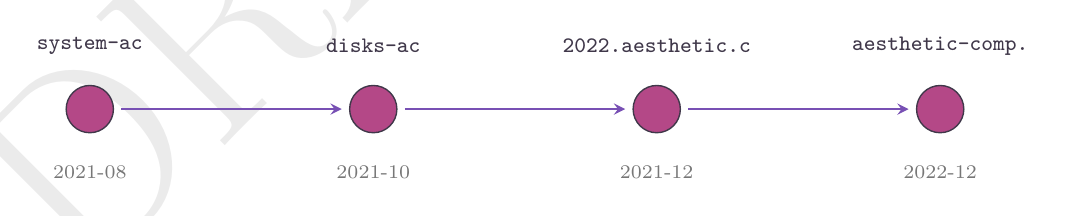
\begin{tikzpicture}[x=1mm,y=1mm]
  \definecolor{lpink}{RGB}{180,72,135}
  \definecolor{lpurple}{RGB}{120,80,180}
  \definecolor{ldark}{RGB}{64,56,74}
  \definecolor{lgray}{RGB}{119,119,119}
  \draw[->,>=stealth,line width=0.8pt,lpurple] (22,14) -- (50,14);
  \draw[->,>=stealth,line width=0.8pt,lpurple] (58,14) -- (86,14);
  \draw[->,>=stealth,line width=0.8pt,lpurple] (94,14) -- (122,14);
  \fill[lpink] (18,14) circle (3);
  \draw[ldark,line width=0.5pt] (18,14) circle (3);
  \node[font=\footnotesize\color{ldark}] at (18,22) {\texttt{system-ac}};
  \node[font=\scriptsize\color{lgray}] at (18,6) {2021-08};
  \fill[lpink] (54,14) circle (3);
  \draw[ldark,line width=0.5pt] (54,14) circle (3);
  \node[font=\footnotesize\color{ldark}] at (54,22) {\texttt{disks-ac}};
  \node[font=\scriptsize\color{lgray}] at (54,6) {2021-10};
  \fill[lpink] (90,14) circle (3);
  \draw[ldark,line width=0.5pt] (90,14) circle (3);
  \node[font=\footnotesize\color{ldark}] at (90,22) {\texttt{2022.aesthetic.c}};
  \node[font=\scriptsize\color{lgray}] at (90,6) {2021-12};
  \fill[lpink] (126,14) circle (3);
  \draw[ldark,line width=0.5pt] (126,14) circle (3);
  \node[font=\footnotesize\color{ldark}] at (126,22) {\texttt{aesthetic-comp.}};
  \node[font=\scriptsize\color{lgray}] at (126,6) {2022-12};
\end{tikzpicture}

\caption{The four successive AC repositories in chronological order, generated from the static lineage table imported by \texttt{build-figures.mjs}. The same substance compiles via Penrose to a force-laid SVG; we ship the TikZ fallback here so the paper builds in CI without the Penrose toolchain.}
\label{fig:lineage}
\end{figure}

Figure~\ref{fig:lineage} shows the simplest case: four \texttt{Repo} instances, three \texttt{Succeeds} relations, a horizontal layout. Compare this to the two paragraphs of explicit \texttt{tikz} coordinates one would otherwise write --- the substance is shorter than the picture it produces.

\subsection{KidLisp Categories}

\begin{figure}[h]
\centering
\resizebox{\linewidth}{!}{% generated by build-figures.mjs — DO NOT EDIT
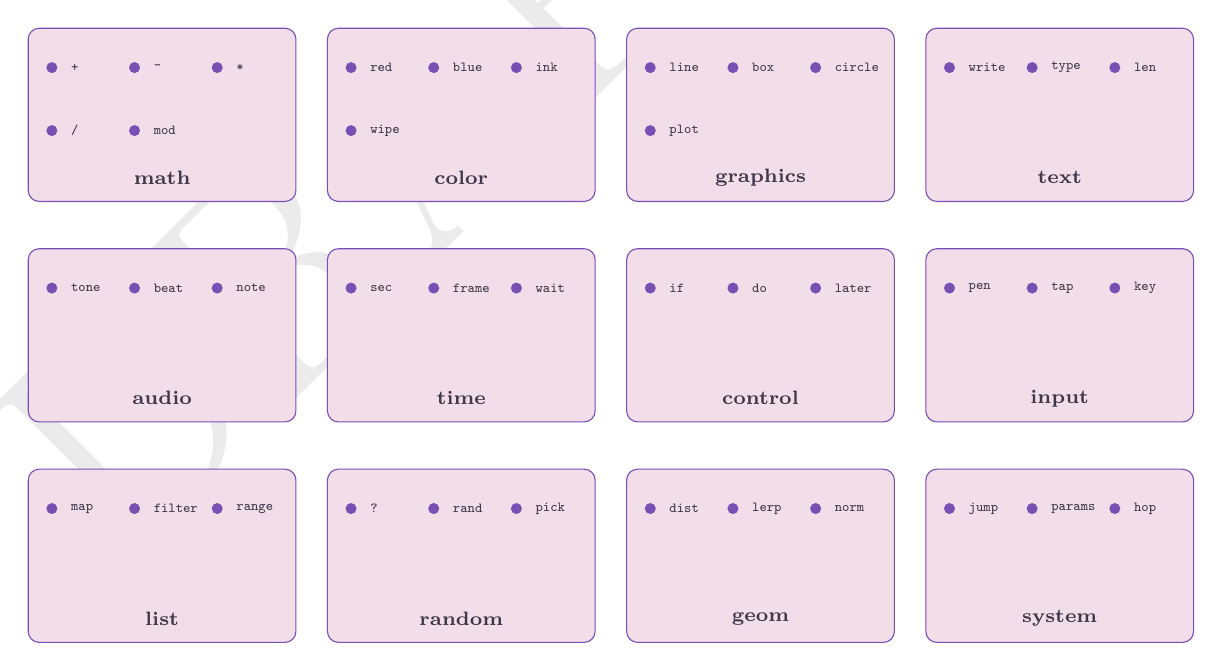
\begin{tikzpicture}[x=1mm,y=1mm]
  \definecolor{lpink}{RGB}{180,72,135}
  \definecolor{lpurple}{RGB}{120,80,180}
  \definecolor{ldark}{RGB}{64,56,74}
  \draw[lpurple,fill=lpink!18,line width=0.4pt,rounded corners=1.4mm] (4,-6) rectangle (38,-28);
  \node[font=\scriptsize\bfseries\color{ldark}] at (21,-25) {math};
  \fill[lpurple] (7,-11) circle (0.7);
  \node[font=\tiny\color{ldark},anchor=west] at (8.2,-11) {\texttt{+}};
  \fill[lpurple] (17.5,-11) circle (0.7);
  \node[font=\tiny\color{ldark},anchor=west] at (18.7,-11) {\texttt{-}};
  \fill[lpurple] (28,-11) circle (0.7);
  \node[font=\tiny\color{ldark},anchor=west] at (29.2,-11) {\texttt{*}};
  \fill[lpurple] (7,-19) circle (0.7);
  \node[font=\tiny\color{ldark},anchor=west] at (8.2,-19) {\texttt{/}};
  \fill[lpurple] (17.5,-19) circle (0.7);
  \node[font=\tiny\color{ldark},anchor=west] at (18.7,-19) {\texttt{mod}};
  \draw[lpurple,fill=lpink!18,line width=0.4pt,rounded corners=1.4mm] (42,-6) rectangle (76,-28);
  \node[font=\scriptsize\bfseries\color{ldark}] at (59,-25) {color};
  \fill[lpurple] (45,-11) circle (0.7);
  \node[font=\tiny\color{ldark},anchor=west] at (46.2,-11) {\texttt{red}};
  \fill[lpurple] (55.5,-11) circle (0.7);
  \node[font=\tiny\color{ldark},anchor=west] at (56.7,-11) {\texttt{blue}};
  \fill[lpurple] (66,-11) circle (0.7);
  \node[font=\tiny\color{ldark},anchor=west] at (67.2,-11) {\texttt{ink}};
  \fill[lpurple] (45,-19) circle (0.7);
  \node[font=\tiny\color{ldark},anchor=west] at (46.2,-19) {\texttt{wipe}};
  \draw[lpurple,fill=lpink!18,line width=0.4pt,rounded corners=1.4mm] (80,-6) rectangle (114,-28);
  \node[font=\scriptsize\bfseries\color{ldark}] at (97,-25) {graphics};
  \fill[lpurple] (83,-11) circle (0.7);
  \node[font=\tiny\color{ldark},anchor=west] at (84.2,-11) {\texttt{line}};
  \fill[lpurple] (93.5,-11) circle (0.7);
  \node[font=\tiny\color{ldark},anchor=west] at (94.7,-11) {\texttt{box}};
  \fill[lpurple] (104,-11) circle (0.7);
  \node[font=\tiny\color{ldark},anchor=west] at (105.2,-11) {\texttt{circle}};
  \fill[lpurple] (83,-19) circle (0.7);
  \node[font=\tiny\color{ldark},anchor=west] at (84.2,-19) {\texttt{plot}};
  \draw[lpurple,fill=lpink!18,line width=0.4pt,rounded corners=1.4mm] (118,-6) rectangle (152,-28);
  \node[font=\scriptsize\bfseries\color{ldark}] at (135,-25) {text};
  \fill[lpurple] (121,-11) circle (0.7);
  \node[font=\tiny\color{ldark},anchor=west] at (122.2,-11) {\texttt{write}};
  \fill[lpurple] (131.5,-11) circle (0.7);
  \node[font=\tiny\color{ldark},anchor=west] at (132.7,-11) {\texttt{type}};
  \fill[lpurple] (142,-11) circle (0.7);
  \node[font=\tiny\color{ldark},anchor=west] at (143.2,-11) {\texttt{len}};
  \draw[lpurple,fill=lpink!18,line width=0.4pt,rounded corners=1.4mm] (4,-34) rectangle (38,-56);
  \node[font=\scriptsize\bfseries\color{ldark}] at (21,-53) {audio};
  \fill[lpurple] (7,-39) circle (0.7);
  \node[font=\tiny\color{ldark},anchor=west] at (8.2,-39) {\texttt{tone}};
  \fill[lpurple] (17.5,-39) circle (0.7);
  \node[font=\tiny\color{ldark},anchor=west] at (18.7,-39) {\texttt{beat}};
  \fill[lpurple] (28,-39) circle (0.7);
  \node[font=\tiny\color{ldark},anchor=west] at (29.2,-39) {\texttt{note}};
  \draw[lpurple,fill=lpink!18,line width=0.4pt,rounded corners=1.4mm] (42,-34) rectangle (76,-56);
  \node[font=\scriptsize\bfseries\color{ldark}] at (59,-53) {time};
  \fill[lpurple] (45,-39) circle (0.7);
  \node[font=\tiny\color{ldark},anchor=west] at (46.2,-39) {\texttt{sec}};
  \fill[lpurple] (55.5,-39) circle (0.7);
  \node[font=\tiny\color{ldark},anchor=west] at (56.7,-39) {\texttt{frame}};
  \fill[lpurple] (66,-39) circle (0.7);
  \node[font=\tiny\color{ldark},anchor=west] at (67.2,-39) {\texttt{wait}};
  \draw[lpurple,fill=lpink!18,line width=0.4pt,rounded corners=1.4mm] (80,-34) rectangle (114,-56);
  \node[font=\scriptsize\bfseries\color{ldark}] at (97,-53) {control};
  \fill[lpurple] (83,-39) circle (0.7);
  \node[font=\tiny\color{ldark},anchor=west] at (84.2,-39) {\texttt{if}};
  \fill[lpurple] (93.5,-39) circle (0.7);
  \node[font=\tiny\color{ldark},anchor=west] at (94.7,-39) {\texttt{do}};
  \fill[lpurple] (104,-39) circle (0.7);
  \node[font=\tiny\color{ldark},anchor=west] at (105.2,-39) {\texttt{later}};
  \draw[lpurple,fill=lpink!18,line width=0.4pt,rounded corners=1.4mm] (118,-34) rectangle (152,-56);
  \node[font=\scriptsize\bfseries\color{ldark}] at (135,-53) {input};
  \fill[lpurple] (121,-39) circle (0.7);
  \node[font=\tiny\color{ldark},anchor=west] at (122.2,-39) {\texttt{pen}};
  \fill[lpurple] (131.5,-39) circle (0.7);
  \node[font=\tiny\color{ldark},anchor=west] at (132.7,-39) {\texttt{tap}};
  \fill[lpurple] (142,-39) circle (0.7);
  \node[font=\tiny\color{ldark},anchor=west] at (143.2,-39) {\texttt{key}};
  \draw[lpurple,fill=lpink!18,line width=0.4pt,rounded corners=1.4mm] (4,-62) rectangle (38,-84);
  \node[font=\scriptsize\bfseries\color{ldark}] at (21,-81) {list};
  \fill[lpurple] (7,-67) circle (0.7);
  \node[font=\tiny\color{ldark},anchor=west] at (8.2,-67) {\texttt{map}};
  \fill[lpurple] (17.5,-67) circle (0.7);
  \node[font=\tiny\color{ldark},anchor=west] at (18.7,-67) {\texttt{filter}};
  \fill[lpurple] (28,-67) circle (0.7);
  \node[font=\tiny\color{ldark},anchor=west] at (29.2,-67) {\texttt{range}};
  \draw[lpurple,fill=lpink!18,line width=0.4pt,rounded corners=1.4mm] (42,-62) rectangle (76,-84);
  \node[font=\scriptsize\bfseries\color{ldark}] at (59,-81) {random};
  \fill[lpurple] (45,-67) circle (0.7);
  \node[font=\tiny\color{ldark},anchor=west] at (46.2,-67) {\texttt{?}};
  \fill[lpurple] (55.5,-67) circle (0.7);
  \node[font=\tiny\color{ldark},anchor=west] at (56.7,-67) {\texttt{rand}};
  \fill[lpurple] (66,-67) circle (0.7);
  \node[font=\tiny\color{ldark},anchor=west] at (67.2,-67) {\texttt{pick}};
  \draw[lpurple,fill=lpink!18,line width=0.4pt,rounded corners=1.4mm] (80,-62) rectangle (114,-84);
  \node[font=\scriptsize\bfseries\color{ldark}] at (97,-81) {geom};
  \fill[lpurple] (83,-67) circle (0.7);
  \node[font=\tiny\color{ldark},anchor=west] at (84.2,-67) {\texttt{dist}};
  \fill[lpurple] (93.5,-67) circle (0.7);
  \node[font=\tiny\color{ldark},anchor=west] at (94.7,-67) {\texttt{lerp}};
  \fill[lpurple] (104,-67) circle (0.7);
  \node[font=\tiny\color{ldark},anchor=west] at (105.2,-67) {\texttt{norm}};
  \draw[lpurple,fill=lpink!18,line width=0.4pt,rounded corners=1.4mm] (118,-62) rectangle (152,-84);
  \node[font=\scriptsize\bfseries\color{ldark}] at (135,-81) {system};
  \fill[lpurple] (121,-67) circle (0.7);
  \node[font=\tiny\color{ldark},anchor=west] at (122.2,-67) {\texttt{jump}};
  \fill[lpurple] (131.5,-67) circle (0.7);
  \node[font=\tiny\color{ldark},anchor=west] at (132.7,-67) {\texttt{params}};
  \fill[lpurple] (142,-67) circle (0.7);
  \node[font=\tiny\color{ldark},anchor=west] at (143.2,-67) {\texttt{hop}};
\end{tikzpicture}
}
\caption{Twelve KidLisp categories with a sample of their built-ins. Each cell is a \texttt{Category} box laid out by the \texttt{categories.style} solver under a \texttt{contains(c.box, f.dot)} constraint per \texttt{Member} fact. Keys verified against \texttt{kidlisp.mjs} render in mono; absent keys (defined dynamically in the evaluator) are still listed but flagged in build output.}
\label{fig:categories}
\end{figure}

Figure~\ref{fig:categories} is more interesting because the substance contains \emph{set membership} rather than positional information. The style declares \texttt{ensure contains(c.box, f.dot)} for every \texttt{Member(fn, c)} fact and \texttt{ensure disjoint(c1.box, c2.box, 12)} between every pair of categories. Penrose then finds positions that satisfy all constraints simultaneously. In the TikZ fallback we use a fixed grid; the Penrose render trades the grid for a more relaxed embedding.

\subsection{Piece--Library Graph}

\begin{figure}[h]
\centering
\resizebox{\linewidth}{!}{% generated by build-figures.mjs — DO NOT EDIT
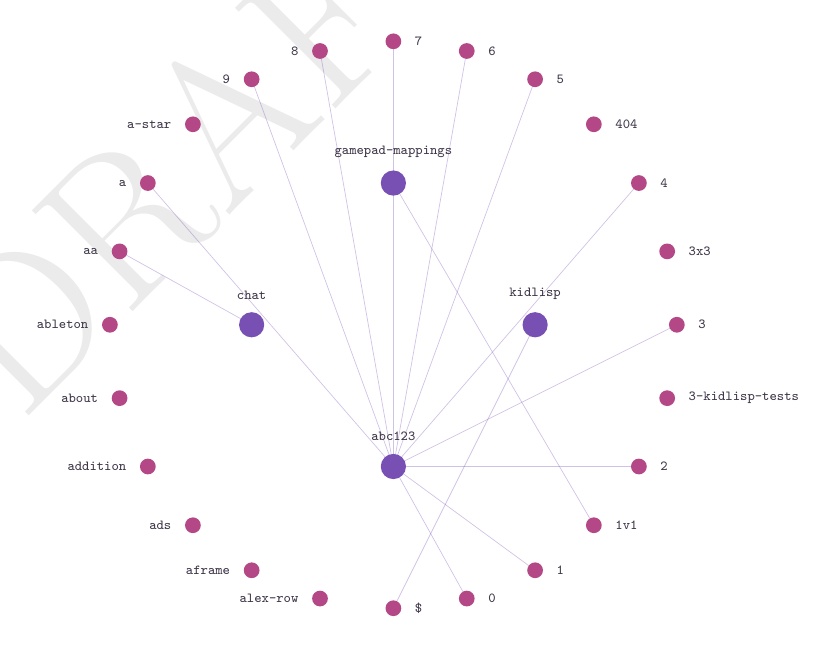
\begin{tikzpicture}[x=1mm,y=1mm]
  \definecolor{lpink}{RGB}{180,72,135}
  \definecolor{lpurple}{RGB}{120,80,180}
  \definecolor{ldark}{RGB}{64,56,74}
  \draw[lpurple,opacity=0.35,line width=0.25pt] (0.00,-36.00) -- (18.00,0.00);
  \draw[lpurple,opacity=0.35,line width=0.25pt] (9.32,-34.77) -- (0.00,-18.00);
  \draw[lpurple,opacity=0.35,line width=0.25pt] (18.00,-31.18) -- (0.00,-18.00);
  \draw[lpurple,opacity=0.35,line width=0.25pt] (25.46,-25.46) -- (0.00,18.00);
  \draw[lpurple,opacity=0.35,line width=0.25pt] (31.18,-18.00) -- (0.00,-18.00);
  \draw[lpurple,opacity=0.35,line width=0.25pt] (36.00,0.00) -- (0.00,-18.00);
  \draw[lpurple,opacity=0.35,line width=0.25pt] (31.18,18.00) -- (0.00,-18.00);
  \draw[lpurple,opacity=0.35,line width=0.25pt] (18.00,31.18) -- (0.00,-18.00);
  \draw[lpurple,opacity=0.35,line width=0.25pt] (9.32,34.77) -- (0.00,-18.00);
  \draw[lpurple,opacity=0.35,line width=0.25pt] (0.00,36.00) -- (0.00,-18.00);
  \draw[lpurple,opacity=0.35,line width=0.25pt] (-9.32,34.77) -- (0.00,-18.00);
  \draw[lpurple,opacity=0.35,line width=0.25pt] (-18.00,31.18) -- (0.00,-18.00);
  \draw[lpurple,opacity=0.35,line width=0.25pt] (-31.18,18.00) -- (0.00,-18.00);
  \draw[lpurple,opacity=0.35,line width=0.25pt] (-34.77,9.32) -- (-18.00,0.00);
  \fill[lpurple] (0.00,-18.00) circle (1.6);
  \node[font=\tiny\color{ldark},anchor=south] at (0.00,-16.00) {\texttt{abc123}};
  \fill[lpurple] (18.00,0.00) circle (1.6);
  \node[font=\tiny\color{ldark},anchor=south] at (18.00,2.00) {\texttt{kidlisp}};
  \fill[lpurple] (0.00,18.00) circle (1.6);
  \node[font=\tiny\color{ldark},anchor=south] at (0.00,20.00) {\texttt{gamepad-mappings}};
  \fill[lpurple] (-18.00,0.00) circle (1.6);
  \node[font=\tiny\color{ldark},anchor=south] at (-18.00,2.00) {\texttt{chat}};
  \fill[lpink] (0.00,-36.00) circle (1.0);
  \node[font=\tiny\color{ldark},anchor=west] at (1.50,-36.00) {\texttt{\$}};
  \fill[lpink] (9.32,-34.77) circle (1.0);
  \node[font=\tiny\color{ldark},anchor=west] at (10.82,-34.77) {\texttt{0}};
  \fill[lpink] (18.00,-31.18) circle (1.0);
  \node[font=\tiny\color{ldark},anchor=west] at (19.50,-31.18) {\texttt{1}};
  \fill[lpink] (25.46,-25.46) circle (1.0);
  \node[font=\tiny\color{ldark},anchor=west] at (26.96,-25.46) {\texttt{1v1}};
  \fill[lpink] (31.18,-18.00) circle (1.0);
  \node[font=\tiny\color{ldark},anchor=west] at (32.68,-18.00) {\texttt{2}};
  \fill[lpink] (34.77,-9.32) circle (1.0);
  \node[font=\tiny\color{ldark},anchor=west] at (36.27,-9.32) {\texttt{3-kidlisp-tests}};
  \fill[lpink] (36.00,0.00) circle (1.0);
  \node[font=\tiny\color{ldark},anchor=west] at (37.50,0.00) {\texttt{3}};
  \fill[lpink] (34.77,9.32) circle (1.0);
  \node[font=\tiny\color{ldark},anchor=west] at (36.27,9.32) {\texttt{3x3}};
  \fill[lpink] (31.18,18.00) circle (1.0);
  \node[font=\tiny\color{ldark},anchor=west] at (32.68,18.00) {\texttt{4}};
  \fill[lpink] (25.46,25.46) circle (1.0);
  \node[font=\tiny\color{ldark},anchor=west] at (26.96,25.46) {\texttt{404}};
  \fill[lpink] (18.00,31.18) circle (1.0);
  \node[font=\tiny\color{ldark},anchor=west] at (19.50,31.18) {\texttt{5}};
  \fill[lpink] (9.32,34.77) circle (1.0);
  \node[font=\tiny\color{ldark},anchor=west] at (10.82,34.77) {\texttt{6}};
  \fill[lpink] (0.00,36.00) circle (1.0);
  \node[font=\tiny\color{ldark},anchor=west] at (1.50,36.00) {\texttt{7}};
  \fill[lpink] (-9.32,34.77) circle (1.0);
  \node[font=\tiny\color{ldark},anchor=east] at (-10.82,34.77) {\texttt{8}};
  \fill[lpink] (-18.00,31.18) circle (1.0);
  \node[font=\tiny\color{ldark},anchor=east] at (-19.50,31.18) {\texttt{9}};
  \fill[lpink] (-25.46,25.46) circle (1.0);
  \node[font=\tiny\color{ldark},anchor=east] at (-26.96,25.46) {\texttt{a-star}};
  \fill[lpink] (-31.18,18.00) circle (1.0);
  \node[font=\tiny\color{ldark},anchor=east] at (-32.68,18.00) {\texttt{a}};
  \fill[lpink] (-34.77,9.32) circle (1.0);
  \node[font=\tiny\color{ldark},anchor=east] at (-36.27,9.32) {\texttt{aa}};
  \fill[lpink] (-36.00,0.00) circle (1.0);
  \node[font=\tiny\color{ldark},anchor=east] at (-37.50,0.00) {\texttt{ableton}};
  \fill[lpink] (-34.77,-9.32) circle (1.0);
  \node[font=\tiny\color{ldark},anchor=east] at (-36.27,-9.32) {\texttt{about}};
  \fill[lpink] (-31.18,-18.00) circle (1.0);
  \node[font=\tiny\color{ldark},anchor=east] at (-32.68,-18.00) {\texttt{addition}};
  \fill[lpink] (-25.46,-25.46) circle (1.0);
  \node[font=\tiny\color{ldark},anchor=east] at (-26.96,-25.46) {\texttt{ads}};
  \fill[lpink] (-18.00,-31.18) circle (1.0);
  \node[font=\tiny\color{ldark},anchor=east] at (-19.50,-31.18) {\texttt{aframe}};
  \fill[lpink] (-9.32,-34.77) circle (1.0);
  \node[font=\tiny\color{ldark},anchor=east] at (-10.82,-34.77) {\texttt{alex-row}};
\end{tikzpicture}
}
\caption{A 24-piece sample (alphabetical, deterministic) and the eight most-imported library modules. Edges are \texttt{Imports} facts mined from each piece's \texttt{from "\ldots/lib/\ldots"} statements. Pink: pieces. Purple: libraries. The TikZ fallback uses concentric rings for legibility; Penrose's force-directed style produces a softer organic embedding.}
\label{fig:clusters}
\end{figure}

Figure~\ref{fig:clusters} is the figure that most needs to be data-driven. The set of pieces and their library dependencies changes weekly; any hand-drawn version of this graph would be wrong by the time the paper is read. The substance file for this figure is regenerated by walking the disks directory and parsing imports --- a $\sim$30-line loop in the build script.

% ============ 5. PIPELINE ============

\section{Pipeline}

\begin{table}[h]
\small
\centering
\begin{tabular}{ll}
\toprule
\textbf{Stage} & \textbf{Tool} \\
\midrule
introspect repo                     & \texttt{node fs.readdirSync, regex} \\
emit \texttt{.substance}            & \texttt{build-figures.mjs}          \\
compile to SVG (optional)           & \texttt{npx @penrose/roger trio}    \\
fallback to TikZ                    & \texttt{build-figures.mjs}          \\
embed in paper                      & \texttt{\textbackslash input\{\ldots.tex\}} \\
\bottomrule
\end{tabular}
\caption{The five-stage build. Stages 1--2 and 4--5 always run; stage 3 runs only when \texttt{npx} can resolve \texttt{@penrose/roger}.}
\end{table}

The full build is one command:

\begin{lstlisting}[language=bash]
node papers/arxiv-penrose/build-figures.mjs
\end{lstlisting}

\noindent which (a) writes \texttt{.substance} files into \texttt{figures/penrose/substance/}, (b) writes deterministic TikZ pictures into \texttt{figures/}, and (c) attempts to compile each Penrose trio to SVG. A failure at stage~(c) is non-fatal --- the TikZ fallback from stage~(b) is what actually makes it into the PDF you are reading.

This matters for CI. The papers stack runs on an oven server~\citep{scudder2026score} that pulls latex but cannot guarantee a Node CDN connection for every build. Shipping the TikZ alongside the Penrose source means the canonical artifact is a live render of repo state, but the paper still compiles cold.

% ============ 6. FUTURE ============

\section{Future Work}

The current pipeline emits static figures. Three near-term extensions are within reach:

\begin{itemize}
  \item \textbf{Live diagrams in pieces.} Penrose's diagrams are SVG; AC pieces can already render SVG via the \texttt{paste} primitive. A piece called \texttt{\$repo-graph} could re-fetch the substance from a backend and render the same illustration the paper uses, but with today's data and tomorrow's data being legibly different.
  \item \textbf{Multiplayer topology.} The \texttt{Player}, \texttt{Session}, \texttt{JoinedSession}, and \texttt{Plays} predicates already exist in the domain but no figure uses them yet. The session server's \texttt{others}/\texttt{everyone} relay distinction~\citep{scudder2026ac} maps cleanly onto two style colors.
  \item \textbf{Citation graph.} The papers stack itself is a graph: papers cite papers, share figures, and cluster by topic. A Penrose substance emitted from \texttt{papermill.mjs sync-index} would draw the graph that the platter currently only describes in prose.
\end{itemize}

Penrose itself is also evolving --- the Bloom~\citep{bloom2024} framework adds animation and interaction on top of the same domain/style separation. An animated lineage diagram, where each new \texttt{Repo} fades in as it is committed, would let the archaeology paper~\citep{scudder2026archaeology} \emph{play} rather than just show.

\section{Conclusion}

Diagrams in research papers usually rot. The pipeline described here treats every illustration as a derived artifact: the source of truth is the repository, the diagram is what falls out of running a script over it. Penrose~\citep{ye2020penrose} provides the declarative layer that makes that approach possible without requiring each paper to own its own layout code. The paper you are reading is its own first reader: if you re-run \texttt{build-figures.mjs} a year from now, the four-repo lineage will still be four repos, but the piece--library graph will have moved.

\vspace{0.5em}
\noindent\textbf{Reproducibility.} Source: \texttt{papers/arxiv-penrose/}. Run \texttt{node build-figures.mjs} for substance + TikZ; add \texttt{@penrose/roger} on PATH for SVG. The figures in this paper were generated from commit \texttt{HEAD} at the time of compile.

\vspace{0.5em}
\noindent\textbf{ORCID:} \href{https://orcid.org/0009-0007-4460-4913}{0009-0007-4460-4913}

% ============ REFERENCES ============

\bibliographystyle{plainnat}
\bibliography{references}

\end{document}
